\section{Blade grinder vibration}
\SectionPage

\begin{frame}
    \frametitle{Intro \& Goals}
    \vspace*{\fill}
    \begin{columns}[onlytextwidth, c]
        \begin{column}{.47\textwidth}
            Improve blade-cutting machine line; has a high number of standstills and not ideal quality of the cut.

            \textbf{General goals}:
            \begin{itemize}
                \item Increase production quality
                \item Avoid unplanned standstill \& extend machines's life
                \item Identify the impact of the grindstones turning
                \item Find the root-cause of strong vibration
            \end{itemize}
        \end{column}
        \begin{column}{.52\textwidth}
            \begin{figure}[ht]
                \begin{subfigure}{\textwidth}
                    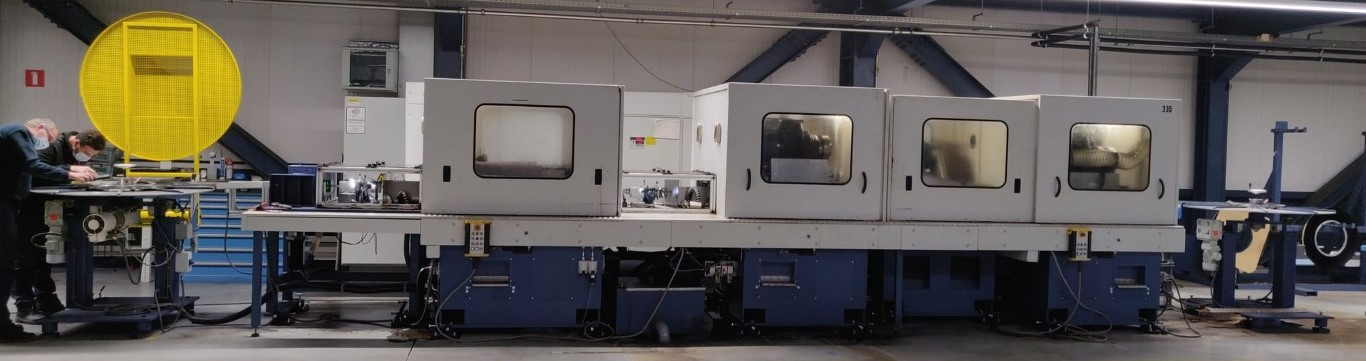
\includegraphics[width=\linewidth]{stumabo/installation/line_photo.jpg}
                    \caption{Line overview: side view}
                    \label{fig:line_overview}
                \end{subfigure}
                \begin{subfigure}{\textwidth}
                    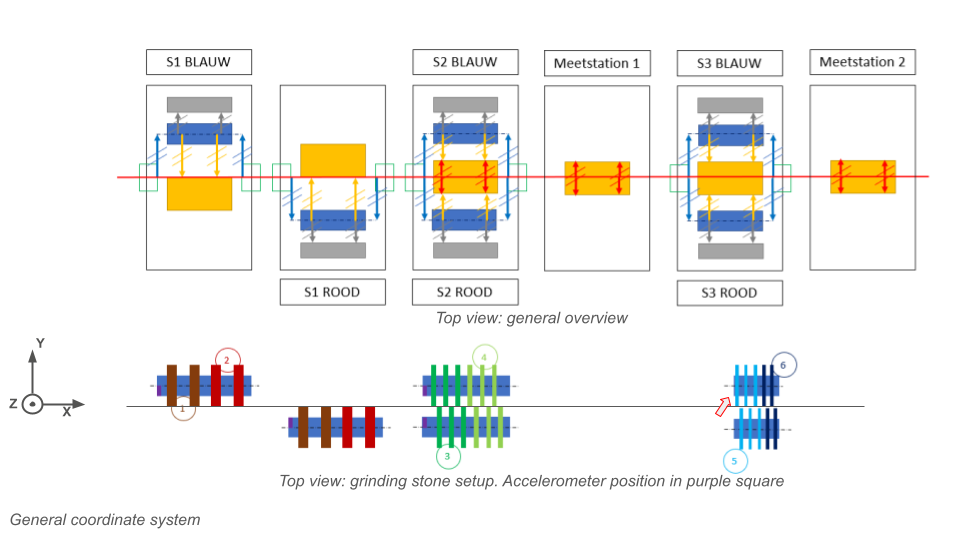
\includegraphics[width=\textwidth]{stumabo/installation/general_cordinate_system.png}
                    \caption{Top view schematics}
                \end{subfigure}
            \end{figure}
        \end{column}
    \end{columns}
    \vspace*{\fill}
\end{frame}

\begin{frame}
    \frametitle{4 Phases -- I}
    \vspace*{\fill}
    \begin{columns}[onlytextwidth, c]
        \begin{column}{.47\textwidth}
            \begin{exampleblock}{Hardware \& Data sources}
                \begin{itemize}
                    \item 3-dimension accelerometer
                    \item mobile cabinet
                    \item log file (operational data)
                \end{itemize}
            \end{exampleblock}
        \end{column}

        \begin{column}{.52\textwidth}
            \begin{figure}[ht]
                \begin{subfigure}{0.49\textwidth}
                    \centering
                    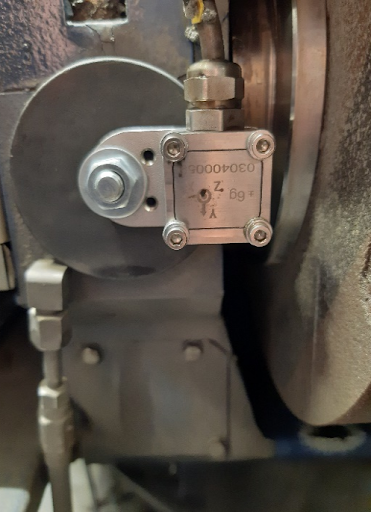
\includegraphics[height=\linewidth]{stumabo/installation/acc_station_1_blue.png}
                    \caption{Installation photo}
                \end{subfigure}
                \begin{subfigure}{0.49\textwidth}
                    \centering
                    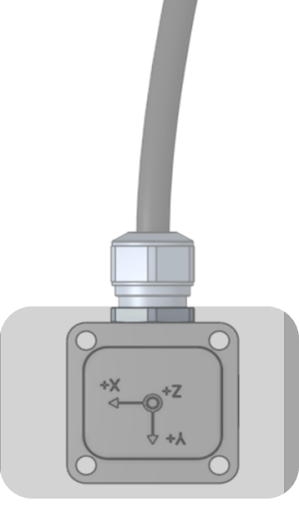
\includegraphics[height=\linewidth]{stumabo/installation/acc_render.png}
                    \caption{CAD render}
                \end{subfigure}
            \end{figure}
        \end{column}
    \end{columns}
    \vspace*{\fill}
\end{frame}

\begin{frame}
    \frametitle{4 Phases -- II}
    \vspace*{\fill}
    \begin{columns}[onlytextwidth, c]
        \begin{column}{.47\textwidth}
            \begin{exampleblock}{Installation}
                \begin{itemize}
                    \item \textcolor{red}{red} and \textcolor{blue}{blue} sides
                    \item local $(x,y,z)$ for each sensor placement
                    \item global $(X,Y,Z)$ for the entire production line
                    \item sensor orientation and installation angle
                \end{itemize}
            \end{exampleblock}
        \end{column}
        \begin{column}{.52\textwidth}
            \begin{figure}
                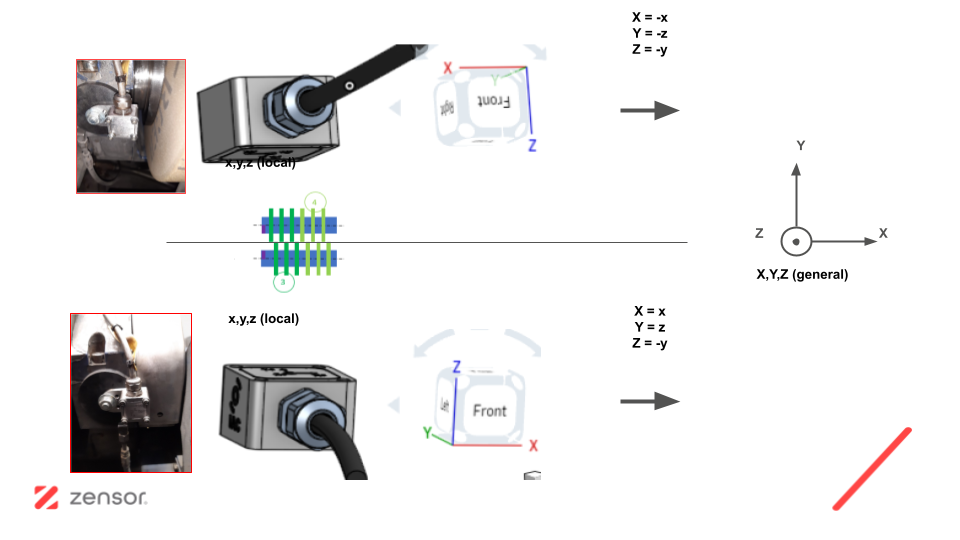
\includegraphics[width=\linewidth]{stumabo/installation/local_to_global.png}
                \caption{From local to general coordinate system}
            \end{figure}
        \end{column}
    \end{columns}
    \vspace*{\fill}
\end{frame}

\begin{frame}
    \frametitle{4 Phases -- III}
    \vspace*{\fill}
    \begin{columns}[onlytextwidth, c]
        \begin{column}{.47\textwidth}
            \begin{exampleblock}{Data Management}
                \begin{itemize}
                    \item single data stream
                    \item  $ ACC_{x, y, z} \longrightarrow DB$ 
                    \item 60Hz to 1Hz /w Lambda
                \end{itemize}
            \end{exampleblock}
        \end{column}
        \begin{column}{.52\textwidth}
            \begin{figure}[ht]
                % Mettere più grandi?
                \begin{subfigure}{\textwidth}
                    \centering
                    \includegraphics[width=.625\textwidth]{stumabo/analysis/60Hz-raw-vibration.pdf}
                    \caption{60Hz raw vibration}
                    \label{fig:stu_60Hz_raw}
                \end{subfigure}
                \begin{subfigure}{\textwidth}
                    \centering
                    \includegraphics[width=.625\textwidth]{stumabo/analysis/1Hz-raw-vibration.pdf}
                    \caption{1Hz raw vibration}
                    \label{fig:stu_1Hz_raw}
                \end{subfigure}
            \end{figure}
        \end{column}
    \end{columns}
    \vspace*{\fill}
\end{frame}

% \begin{figure}
%     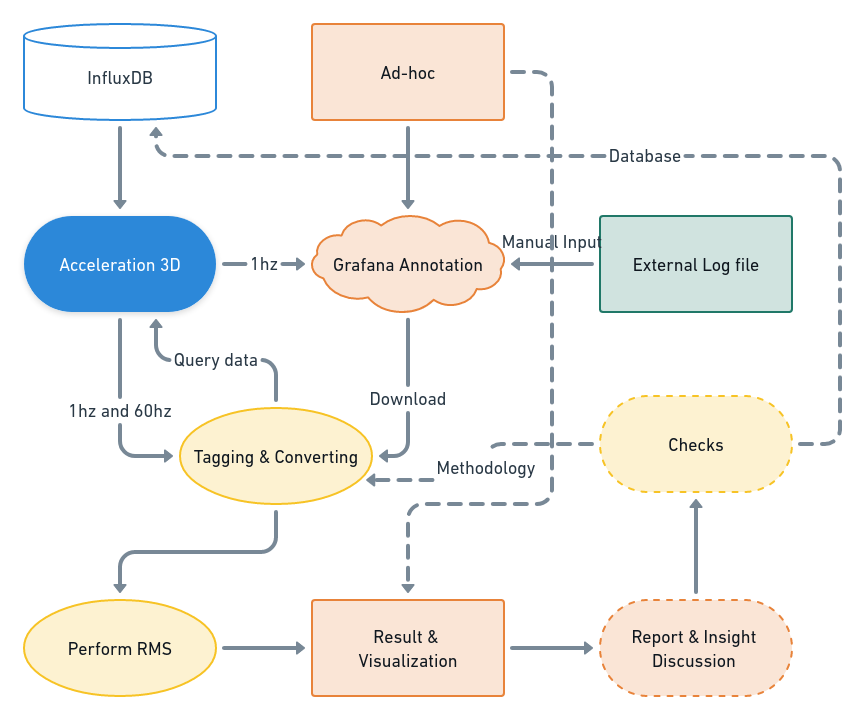
\includegraphics[width=\linewidth]{stumabo/analysis/analysis_flow.png}
%     \caption{Data Management and Analysis overview}
% \end{figure}


\begin{frame}
    \frametitle{Conclusion}
    \vspace*{\fill}

    \vspace*{\fill}
\end{frame}